

\chapter{Resiliencia y futuro del sistema eléctrico}
\label{ch:resiliencia_futuro}

La lección estructural del 28 de abril de 2025 no reside en el colapso en
sí, sino en la clase de vulnerabilidad que reveló. El análisis forense
desarrollado en los capítulos precedentes demostró que el cero de tensión
no fue un fallo de la reserva de potencia activa ni un error puntual de
operación: fue la manifestación terminal de una incompatibilidad de fondo
entre la física de un sistema eléctrico dominado por inversores y un marco
técnico-regulatorio diseñado para redes síncronas. El presente capítulo
traslada esa incompatibilidad al plano prospectivo. La premisa de partida
es que el escenario estructural que propició el 28A ---alta penetración de
Recursos Basados en Inversores
(IBR)\textsuperscript{\ref{anexo:grid_following}}, escasez de generación
síncrona acoplada y una demanda neta deprimida--- no fue una anomalía
climática, sino el anticipo de condiciones que se reproducirán con
frecuencia creciente conforme avance la descarbonización del parque
generador \cite{entsoe2025,futured2024}. La cuestión técnica y regulatoria
que organiza este capítulo es, por tanto, la siguiente: qué
transformaciones ---tecnológicas, normativas y de diseño de mercado---
son necesarias para que un sistema con penetración de IBR superior al
80~\% sea operable con los márgenes de seguridad que el Criterio $N-1$
exige.

% =====================================================================
\section{La física de la fragilidad sistémica: inercia, cortocircuito
y los límites del paradigma \textit{grid-following}}
\label{sec:fisica_fragilidad}
% =====================================================================

\subsection{La degradación de la inercia y la ecuación de oscilación}
\label{subsec:inercia_swing}

La estabilidad dinámica de la frecuencia en un sistema de potencia está
gobernada por la \textit{Ecuación de Oscilación} (\textit{Swing
Equation}), que expresa el balance entre la potencia mecánica aportada
a los ejes de la generación síncrona y la potencia eléctrica extraída
por las cargas:

\begin{equation}
    \frac{2H}{f_0} \, \frac{df}{dt} = P_m - P_e - D \cdot \Delta f
    \label{eq:swing}
\end{equation}

donde $H$ es la constante de inercia equivalente del sistema (en
segundos), $f_0$ la frecuencia nominal de 50~Hz, $df/dt$ la Tasa de
Cambio de Frecuencia (RoCoF)\textsuperscript{\ref{anexo:rocof}}, $P_m$
la potencia mecánica total aportada a los rotores síncronos acoplados,
$P_e$ la potencia eléctrica neta demandada y $D$ el coeficiente de
amortiguamiento de las cargas dependientes de la frecuencia
\cite{nrel2025}.

El parámetro central de la ecuación~\eqref{eq:swing} a efectos del 28A
es $H$: su reducción implica que cualquier desequilibrio de potencia
($P_m - P_e \neq 0$) se traduce en un RoCoF proporcionalmente más agudo,
acortando la ventana temporal disponible para la actuación de los sistemas
de regulación. Los inversores eólicos y solares convencionales ---los
denominados \textit{grid-following}
(GFL)\textsuperscript{\ref{anexo:grid_following}}--- están desacoplados
de la frecuencia de red mediante sus enlaces de corriente continua y no
aportan inercia electromecánica inherente a la
ecuación~\eqref{eq:swing}.

En el momento del cero de tensión, el Operador del Sistema certificó una
inercia disponible de $H = 2{,}3$~s, valor que superaba el umbral de
2{,}0~s recomendado por ENTSO-E \cite{ree2025}. El incidente no fue,
por tanto, un colapso de frecuencia por déficit de masa síncrona: el
RoCoF no superó 1~Hz/s hasta una fase avanzada de la cascada. Este
matiz es determinante para la interpretación prospectiva: el déficit de
inercia no fue la causa del 28A, pero sí el factor estructural que reduce
los márgenes de seguridad del sistema conforme avance la
descarbonización. En escenarios de penetración IBR superior al 80~\%, la
reducción sostenida de $H$ convierte perturbaciones de amplitud moderada
en contingencias de categoría crítica, porque el tiempo disponible antes
de la activación de los relés de deslastre de
carga\textsuperscript{\ref{anexo:ufls}} (UFLS) se comprime hasta
hacerlos inoperables a la velocidad mecánica de apertura de los
interruptores \cite{mitceepr2025}.

\subsection{El colapso del cortocircuito: la métrica de fortaleza de red}
\label{subsec:scr_weakness}

La segunda dimensión de la fragilidad sistémica, y la más directamente
vinculada al mecanismo causal del 28A, es la degradación de la Potencia
de Cortocircuito ($S_{sc}$) en los nudos de la red. Esta magnitud
refleja su capacidad para inyectar corrientes masivas ante faltas,
sostener el perfil de tensión ante variaciones de carga y garantizar el
correcto funcionamiento de las protecciones de distancia y
sobreintensidad.

Un generador síncrono convencional puede inyectar corrientes de
cortocircuito de entre 5 y 7 veces su valor nominal durante los
primeros ciclos de un transitorio. Los inversores, por el contrario,
limitan la inyección de corriente de falta a valores de entre 1{,}1
y 1{,}2~p.u.\textsuperscript{\ref{anexo:pu}} para evitar la fusión de
los semiconductores. Esta diferencia afecta estructuralmente a la
rigidez eléctrica de los nudos y al funcionamiento de las protecciones
\cite{nrel2025,icai2025}.

La parametrización habitual de esta pérdida de capacidad es el
\textit{Short Circuit Ratio}\textsuperscript{\ref{anexo:potencia_cortocircuito}}
(SCR), definido en el Punto de Conexión Común (PCC) como:

\begin{equation}
    \mathrm{SCR} = \frac{S_{sc,\mathrm{PCC}}}{P_{\mathrm{IBR}}}
    \label{eq:scr}
\end{equation}

donde $S_{sc,\mathrm{PCC}}$ es la potencia de cortocircuito aportada
por el resto del sistema en ese nudo, y $P_{\mathrm{IBR}}$ es la
potencia aparente nominal de la instalación basada en inversores. La
ingeniería de sistemas de potencia clasifica los nudos según este ratio
en tres categorías:

\begin{table}[H]
    \centering
    \caption[Clasificación de la fortaleza de red según el Short Circuit Ratio (SCR).]{%
    Clasificación operativa de la fortaleza de red según el SCR y su
    impacto sobre la estabilidad de los inversores
    \textit{grid-following}. Fuente: Elaboración propia /
    \cite{nrel2025}}
    \vspace{0.3cm}
    \label{tab:scr_clasificacion}
    \small
    \begin{tabularx}{\textwidth}{>{\bfseries}p{3.2cm}
                                  >{\centering\arraybackslash}p{2.2cm}
                                  X}
    \toprule
    \textbf{Categoría} & \textbf{Umbral} & \textbf{Implicación operativa} \\
    \midrule
    Red fuerte
        & $\mathrm{SCR} > 3$
        & Los inversores GFL operan con estabilidad de pequeña señal.
          Las protecciones de distancia mantienen selectividad. \\
    \addlinespace
    Red débil
        & $2 \leq \mathrm{SCR} \leq 3$
        & Degradación del margen de estabilidad del PLL ante
          perturbaciones rápidas. Riesgo de interacción adversa entre
          lazos de control de instalaciones próximas. \\
    \addlinespace
    Red muy débil
        & $\mathrm{SCR} < 2$
        & Los PLLs de los inversores GFL exhiben propensión a la
          pérdida de sincronismo ante variaciones de tensión menores.
          Las protecciones de distancia pierden direccionalidad. \\
    \bottomrule
    \end{tabularx}
\end{table}

Durante las horas previas al colapso del 28 de abril, amplias zonas de
la Península Ibérica operaban como ``redes muy débiles'' con valores de
SCR inferiores a 2. La causa era estructural: la producción masiva de
energía solar había desplazado por orden de mérito a las centrales de
ciclo combinado de gas y cogeneración, cuya desconexión eliminó
precisamente las fuentes de $S_{sc}$ que dan rigidez a los nudos de la
red de transporte \cite{nrel2025,icai2025}. En estas condiciones, el
desvío aproximado de tensión en un nudo de transmisión obedece a:

\begin{equation}
    \Delta V \approx \frac{R_{\mathrm{grid}} \cdot P +
                          X_{\mathrm{grid}} \cdot Q}{V_{\mathrm{nom}}}
    \label{eq:delta_v}
\end{equation}

En redes de transporte de altísima tensión (ATT), donde la relación
$X/R$ es habitualmente elevada, la tensión es gobernada
fundamentalmente por la potencia reactiva $Q$. Sin embargo, cuando
$\mathrm{SCR} \ll 2$, la impedancia global $Z_{\mathrm{grid}}$ se hace
tan alta que la magnitud de la tensión pasa a ser también sensible a
variaciones de potencia activa $P$: las rampas de inyección solar
adquieren un poder de perturbación de tensión que en redes síncronas
convencionales resultaría inofensivo \cite{nrel2025}.

\begin{figure}[H]
    \centering
    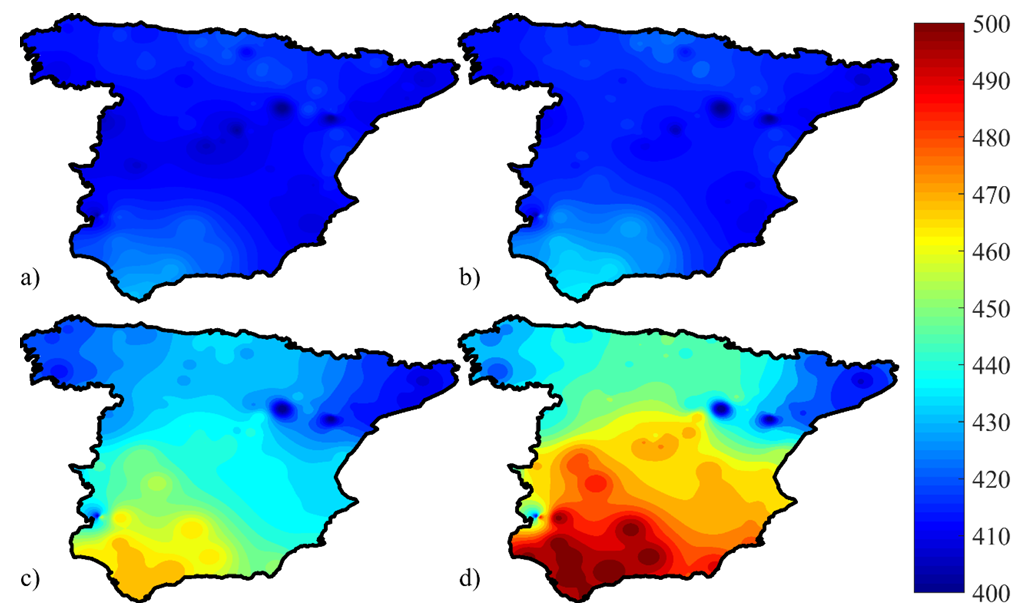
\includegraphics[width=0.90\textwidth]{figuras/scr_iberia.png}
    \vspace{0.2cm}
    \caption[Evolución de las tensiones en la red peninsular de 400~kV
    previa al colapso.]{%
    Mapas de tensión en la red de transporte durante la franja crítica
    previa al colapso (secuencia a--d). Las zonas de color cálido indican
    la progresión y concentración de las sobretensiones severas en el sur
    y suroeste peninsular. Fuente: Informe pericial IIT-ICAI
    \cite{icai2025}.}
    \label{fig:scr_iberia}
\end{figure}

La figura~\ref{fig:scr_iberia} ilustra la evolución geográfica de las
tensiones en la red peninsular de 400~kV en la franja previa al colapso,
tal como fue reconstituida a partir del análisis pericial del IIT-ICAI.
La secuencia evidencia que las sobretensiones más pronunciadas se
concentraron precisamente en aquellos nudos que presentaban una deficiencia
estructural de potencia de cortocircuito, demostrando de forma empírica la
alta sensibilidad a variaciones de tensión en áreas con un SCR bajo.

\subsection{La paradoja geométrica de los inversores: la restricción
\texorpdfstring{$S_{\max}$}{Smax} y el conflicto P-Q}
\label{subsec:smax_conflicto}

La limitación física de los inversores ante condiciones de red débil no
se restringe a la corriente de cortocircuito. Existe una segunda
contradicción estructural, inherente a la geometría del triángulo de
potencia, que el incidente del 28A hizo evidente.

La capacidad aparente máxima de un inversor está acotada por su curva de
capacidad térmica:

\begin{equation}
    S_{\max} = \sqrt{P^2 + Q^2}
    \label{eq:smax}
\end{equation}

Cuando una extensa planta fotovoltaica experimenta un aclaramiento brusco
de nubosidad, sus algoritmos de seguimiento del punto de máxima potencia
(MPPT) ordenan rampas de inyección de potencia activa $P$ de orden de
miles de megavatios por hora. Para no superar el límite térmico del
inversor ($S_{\max}$), el controlador debe reducir simultáneamente su
margen de inyección o absorción de potencia reactiva $Q$. La paradoja
reside en que ese es exactamente el instante en que el aumento brusco
de $P$ sobre una red con $\mathrm{SCR} < 2$ provoca una sobretensión
severa en los nudos locales, exigiendo al inversor una absorción masiva
de reactiva para contenerla. El inversor se enfrenta así a dos
obligaciones físicas simultáneamente incompatibles: maximizar $P$ por
señal de mercado y maximizar $Q$ por necesidad de estabilidad de tensión
\cite{nrel2025,futured2024}.

Esta contradicción intrínseca de la electrónica de potencia en modo
\textit{grid-following} explica por qué el 28A no fue un colapso de
energía, sino de control: el sistema disponía de recursos suficientes
pero carecía de la arquitectura de control necesaria para movilizarlos
coherentemente.

\subsection{La curva de pato y el efecto oculto del autoconsumo
distribuido}
\label{subsec:duck_curve}

El análisis cuantitativo de la secuencia del 28A sitúa el escenario
operativo en el valle profundo de la denominada ``curva de
pato''\textsuperscript{\ref{anexo:duck_curve}} (\textit{duck curve}): la
demanda bruta de ese lunes de abril era estructuralmente baja ---análoga
a los mínimos de hace dos décadas--- mientras que la irradiación
registraba niveles próximos a los máximos estivales por la menor
degradación térmica de las células fotovoltaicas en un día de primavera.

\begin{figure}[H]
    \centering
    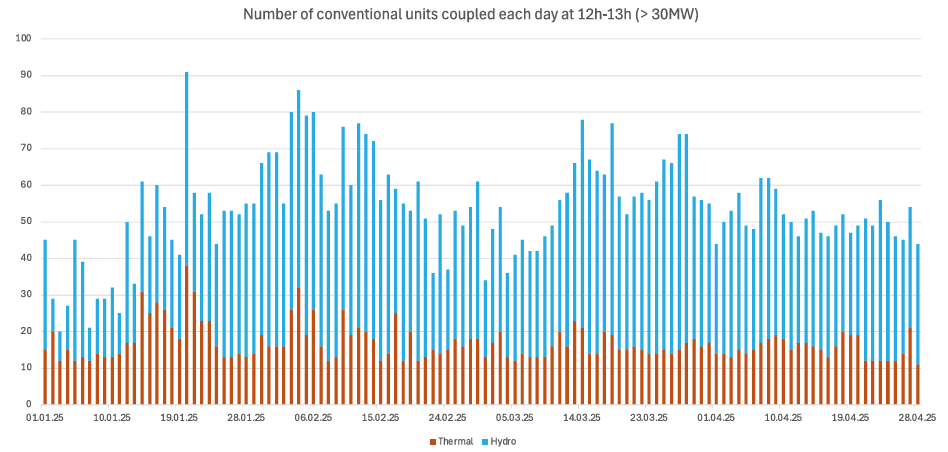
\includegraphics[width=0.90\textwidth]{figuras/conventionalunits.png}
    \vspace{0.2cm}
    \caption[Evolución del acoplamiento de unidades síncronas en horas
    centrales (12h--13h).]{%
    Número de unidades síncronas convencionales acopladas a la red
    diariamente entre las 12h y las 13h. Se evidencia una tendencia
    decreciente en los meses previos al 28 de abril, producto del profundo
    valle de demanda neta (efecto \textit{duck curve}). Esta expulsión por
    orden de mérito vació al sistema de inercia electromecánica en el
    instante crítico. Fuente: ENTSO-E / Elaboración propia.}
    \label{fig:duck_curve}
\end{figure}

A las 12:30~CEST, la generación total del sistema se situaba en
33.612~MW, con la cuota de tecnologías rotativas síncronas reducida a
un mínimo histórico. REE había agotado sus herramientas de gestión
manual ---apertura preventiva de decenas de líneas de muy alta tensión
para aumentar artificialmente la impedancia en serie y reducir la
aportación capacitiva de la red vacía, más la operación de las
reactancias al 85~\% de su capacidad--- sin lograr contener el ascenso
de tensión \cite{icai2025,gobierno2025}.

Un factor adicional que el análisis forense identificó como relevante fue
el comportamiento del autoconsumo fotovoltaico distribuido. El despliegue
masivo de instalaciones de autoconsumo introduce una variable de
incertidumbre estocástica: esta generación detrae demanda visible sin
ser observable telemáticamente a la resolución temporal necesaria.
Durante los fenómenos oscilatorios previos al colapso, las fluctuaciones
de tensión activaron los relés antiislamiento de instalaciones domésticas
e industriales ligeras que, al detectar desviaciones dentro de sus
umbrales de protección, se desconectaron en bloque \cite{mitceepr2025}.
Este evento eliminó de forma instantánea la generación distribuida local,
haciendo aflorar súbitamente la demanda que dichas instalaciones estaban
cubriendo: el efecto fue equivalente a un escalón positivo de carga no
anticipado, en un instante en que el sistema ya carecía de margen de
reactiva para absorber el consiguiente descenso de tensión
\cite{mitceepr2025,gobierno2025}.

La interacción entre la debilidad de red creciente ($\mathrm{SCR} < 2$),
la arquitectura de control \textit{grid-following} de los IBR y la
variabilidad ultrarrápida del recurso solar configura un conjunto de
vulnerabilidades cuya combinación supera la capacidad de los mecanismos
de defensa diseñados para sistemas síncronos convencionales. Esta
interacción es la que el presente capítulo trata de abordar en sus
dimensiones tecnológica, normativa y económica.

% =====================================================================
\section{Tecnologías habilitadoras libres de emisiones: BESS con
capacidad \textit{grid-forming}, compensadores síncronos e inercia
sintética}
\label{sec:tecnologias_habilitadoras}
% =====================================================================

La superación de la vulnerabilidad sistémica evidenciada por el colapso
del 28 de abril exige una transición en la arquitectura de control de la
red: el desplazamiento desde un parque de generación dominado por
dispositivos que \textit{siguen} la tensión y la frecuencia de la red
hacia una infraestructura capaz de \textit{formarlas} de forma autónoma.
En un escenario de descarbonización avanzada, la resiliencia del sistema
depende de la integración de tres familias tecnológicas complementarias.

\vspace{0.4cm}
\noindent\textbf{BESS con control \textit{grid-forming}: velocidad y
precisión.}

A diferencia del inversor \textit{grid-following}, un inversor
\textit{grid-forming}
(GFM)\textsuperscript{\ref{anexo:bess_gfm}} opera como un equivalente
de Thévenin: sintetiza de forma autónoma una referencia interna de tensión
en magnitud y ángulo ($V\angle\delta$) detrás de una impedancia virtual de
acoplamiento. Al imponer este vector de tensión de forma instantánea, el
inversor GFM inyecta o absorbe corriente activa y reactiva de forma
inherente ante cualquier variación de la red, sin depender de mediciones
externas de fase ni de retardos de cálculo
\cite{entsoe2025phase2,nrel2025}.

La figura~\ref{fig:gfl_vs_gfm_circuit1} recoge los circuitos equivalentes
de ambas topologías: el inversor GFL como fuente de corriente con
dependencia del PLL en el PCC, y el inversor GFM como fuente de tensión
autónoma detrás de $Z_{\mathrm{GFM}}$.

\begin{figure}[H]
    \centering
    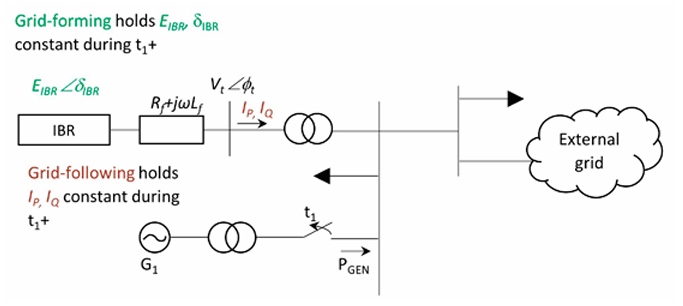
\includegraphics[width=0.85\textwidth]{figuras/gfl_vs_gfm_circuit1.png}
    \vspace{0.2cm}
    \caption[Circuitos equivalentes de las topologías \textit{Grid-Following}
    (GFL) y \textit{Grid-Forming} (GFM).]{%
    Representación unifilar de los circuitos equivalentes para las dos
    topologías de control de inversores. Izquierda: inversor GFL como
    fuente de corriente controlada dependiente del PLL. Derecha: inversor
    GFM como fuente de tensión autónoma detrás de una impedancia virtual
    $Z_{\mathrm{GFM}}$. Fuente: Elaboración propia / Adaptado de
    \cite{nrel2025}}
    \label{fig:gfl_vs_gfm_circuit1}
\end{figure}

Cuando el inversor GFM está respaldado por un banco de baterías
(\textit{BESS-GFM})\textsuperscript{\ref{anexo:bess_gfm}}, la
combinación permite proveer dos servicios adicionales de estabilidad. El
primero es la \textit{inercia
sintética}\textsuperscript{\ref{anexo:inercia_sintetica}}: el algoritmo
de control mide continuamente $df/dt$ y ajusta la potencia de salida de
forma proporcional, liberando o absorbiendo energía del banco en el rango
de decenas de milisegundos, emulando el comportamiento de una masa
rotatoria. El segundo es la \textit{Respuesta Rápida de Frecuencia}
(FFR)\textsuperscript{\ref{anexo:ffr}}: ante la superación de un umbral
de RoCoF o de desviación de frecuencia, el BESS inyecta un bloque de
potencia activa predefinido de forma subcíclica, frenando la pendiente
de caída antes de que los reguladores de velocidad de los grupos síncronos
convencionales hayan podido procesar la perturbación
\cite{nrel2025,futured2024}.

La experiencia operativa de ERCOT (Texas) ilustra los parámetros
cuantitativos de este servicio en un entorno de alta penetración IBR.
ERCOT calcula en tiempo real la inercia del sistema mediante:

\begin{equation}
    M_{\mathrm{sys}} = \sum_{i} H_i \cdot \mathrm{MVA}_i
    \label{eq:ercot_inercia}
\end{equation}

El umbral de inercia crítica estructural se sitúa en torno a
100.000~MW$\cdot$s: por debajo de este nivel, el RoCoF ante una
contingencia de categoría~C (disparo dual de unidades nucleares,
$\approx$~2.750~MW) hunde la frecuencia por debajo de 59{,}3~Hz antes
de que los gobernadores mecánicos convencionales puedan actuar. El
sistema de alarmas establece tres zonas:

\begin{itemize}
    \item \textbf{Zona verde (operación holgada):}
    $M_{\mathrm{sys}} > 120.000$~MW$\cdot$s.
    \item \textbf{Zona amarilla (alerta evolutiva):} entre
    110.000~MW$\cdot$s y 119.999~MW$\cdot$s. Se intensifica la
    monitorización predictiva meteorológica.
    \item \textbf{Zona roja (umbral crítico):}
    $M_{\mathrm{sys}} \leq 100.000$~MW$\cdot$s. El operador fuerza el
    despacho fuera de orden de mérito de unidades síncronas para
    restablecer la masa cinética.
\end{itemize}

Para reducir la dependencia de ese despacho forzado, ERCOT desarrolló
el mercado \textit{Responsive Reserve Service -- Fast Frequency Response}
(RRS-FFR), provisto por sistemas BESS y grandes cargas industriales con
relés de respuesta rápida. Los parámetros de cualificación son los
siguientes: detección autónoma de caída por debajo de 59{,}85~Hz;
inyección del 100~\% de la potencia contratada en un máximo de 15 ciclos
de red (0{,}25~s a 60~Hz); mantenimiento de la inyección entre el 95~\%
y el 110~\% del bloque licitado durante 15~minutos mínimos. Los
resultados operativos verificados muestran que la integración de
450~MW bajo este esquema FFR subcíclico permitió reducir el umbral de
inercia crítica de 100.000~MW$\cdot$s a 88.000~MW$\cdot$s, un descenso
del 12~\% que refleja la equivalencia funcional entre la actuación
sub-segundo de la electrónica de potencia y la masa cinética de las
máquinas síncronas convencionales \cite{futured2024,nrel2025}.

No obstante, la electrónica de potencia presenta una limitación física
estructural: los semiconductores IGBT raramente pueden sostener
corrientes superiores a 1{,}2--1{,}5 veces su valor nominal sin activar
sus protecciones térmicas. Esta restricción implica que la contribución
de los BESS-GFM a la potencia de cortocircuito disponible en el nudo es
cuantitativamente limitada, lo que puede traducirse en una rigidez nodal
insuficiente para el correcto funcionamiento de las protecciones de
distancia ---condición que el IIT-ICAI documentó para el 28A
\cite{icai2025}.

\vspace{0.4cm}
\noindent\textbf{Compensadores síncronos: potencia de cortocircuito e
inercia rotacional genuina.}

La limitación de corriente de los inversores justifica el despliegue
complementario de \textit{compensadores
síncronos}\textsuperscript{\ref{anexo:syncon}} (SynCons): máquinas
rotativas de gran masa acopladas síncronamente a la red pero operadas en
vacío, que intercambian libremente potencia reactiva en función del
nivel de excitación. Su aportación es doble.

El primer aporte es la potencia de
cortocircuito\textsuperscript{\ref{anexo:potencia_cortocircuito}}: los
SynCons pueden inyectar corrientes de cortocircuito del orden del
300--400~\% de su valor nominal durante los primeros ciclos de un
transitorio, incrementando el SCR en el nudo de conexión y dotándolo de
la rigidez eléctrica necesaria para que las protecciones operen
correctamente y para que los IBR próximos puedan mantener el sincronismo
de sus PLL \cite{nrel2025,futured2024}.

El segundo aporte es la inercia rotacional genuina: la energía cinética
almacenada en las masas rotatorias de un SynCon está físicamente
disponible en el primer milisegundo de un transitorio, sin mediación de
algoritmo ni latencia de control, ralentizando el RoCoF de forma
inmediata y ampliando el margen temporal para la actuación de los sistemas
de electrónica de potencia más rápidos. La complementariedad entre la
velocidad y precisión de los BESS-GFM y la robustez y corriente de
cortocircuito de los SynCons define la arquitectura técnica adecuada para
redes en transición avanzada \cite{futured2024}.

\vspace{0.4cm}
\noindent\textbf{La estrategia \textit{Brownfield}: reconversión de
infraestructura fósil clausurada.}

Desde la perspectiva de la viabilidad económica, la literatura de
ingeniería propone una vía de despliegue que minimiza la inversión en
nueva obra civil: la reconversión de instalaciones fósiles clausuradas
en compensadores síncronos, conocida como estrategia
\textit{Brownfield}\textsuperscript{\ref{anexo:brownfield}}. Los grandes
alternadores de las centrales de carbón, ciclo combinado o nuclear en
proceso de desmantelamiento presentan características electromecánicas
---potencia aparente, reactancia transitoria, constante de inercia---
directamente aprovechables para la función de compensación síncrona,
una vez desacoplado el conjunto turbina-generador. Esta reconversión
transforma activos varados en recursos de estabilidad sistémica al tiempo
que conserva el valor de los nudos de evacuación de 400~kV ya instalados
\cite{futured2024,gobierno2025}.

\vspace{0.4cm}
\noindent\textbf{Arquitectura híbrida: la complementariedad como
condición de resiliencia.}

El análisis conjunto de las tres familias tecnológicas permite formular
la conclusión en la que los informes periciales del 28A convergen:
ninguna de ellas, desplegada de forma aislada, es suficiente. Los
BESS-GFM proveen velocidad de respuesta, precisión de control y
capacidad de arranque autónomo en isla (\textit{Black Start}), pero
están limitados en corriente de cortocircuito. Los SynCons proveen
inercia rotacional genuina y potencia de cortocircuito elevada, pero
carecen de la agilidad subcíclica de la electrónica de potencia y no
gestionan energía activa. La inercia sintética y la FFR maximizan la
utilización del margen energético del banco de baterías, pero dependen
de la existencia de una rigidez nodal mínima ---provista por los
SynCons--- para que sus algoritmos de control sean efectivos
\cite{futured2024,nrel2025}.

\begin{figure}[H]
    \centering
    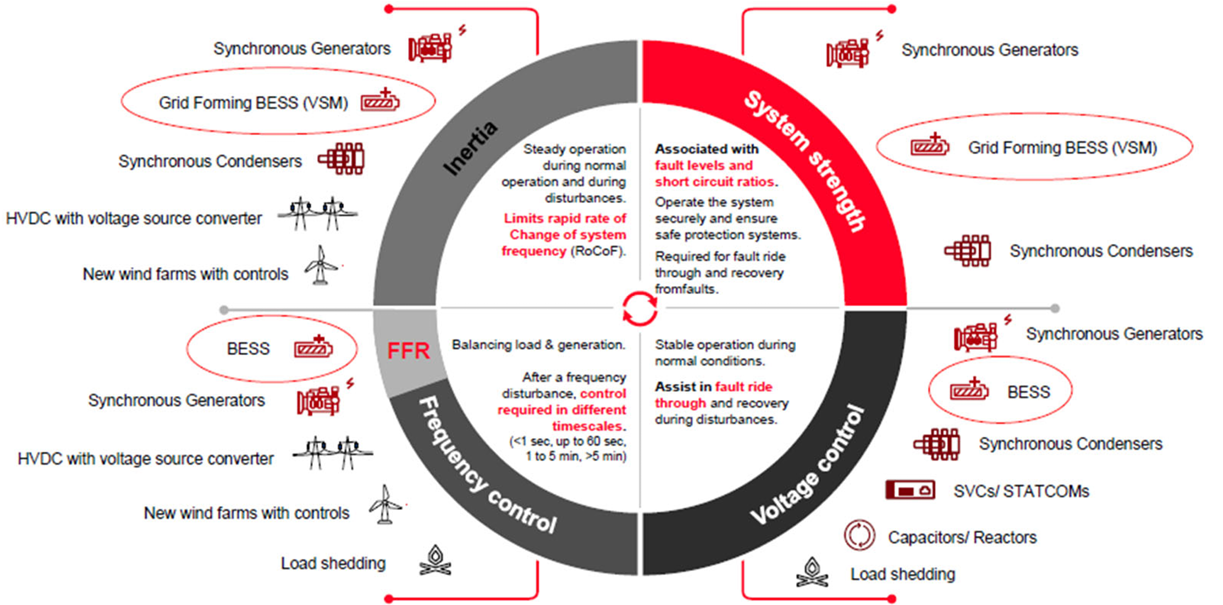
\includegraphics[width=0.80\textwidth]{figuras/hitachi_hybrid.png}
    \vspace{0.2cm}
    \caption[Arquitectura híbrida para la resiliencia sistémica en redes
    descarbonizadas.]{%
    Esquema de la arquitectura híbrida propuesta para redes de alta
    penetración de IBR: los BESS-GFM gestionan la tensión en tiempo real
    y proveen FFR, mientras los compensadores síncronos aportan inercia
    rotacional y potencia de cortocircuito para la rigidez nodal.
    Fuente: Hitachi Energy / Plataforma FUTURED \cite{futured2024}}
    \label{fig:hybrid_architecture}
\end{figure}

La figura~\ref{fig:hybrid_architecture} ilustra la complementariedad:
la resiliencia en un escenario de alta penetración de IBR requiere
combinar el despliegue distribuido de BESS-GFM en nudos de red con la
instalación estratégica de SynCons en los enclaves de mayor exposición
a condiciones de red débil, manteniendo el SCR disponible por encima de
los umbrales que garantizan la operación estable de los IBR y la
fiabilidad de las protecciones. Esta arquitectura no es un paradigma
provisional, sino la solución estructural que la física del sistema
eléctrico descarbonizado impone \cite{gobierno2025,entsoe2025}.

La figura~\ref{fig:futured_coste_optimo} ilustra la consecuencia
económica de este diagnóstico: la minimización del coste total del
sistema no coincide con la minimización del Coste Nivelado de la Energía
(\textit{LCOE})\textsuperscript{\ref{anexo:lcoe}}, sino que exige
internalizar en el diseño de mercado los Servicios Esenciales de
Confiabilidad (ERS)\textsuperscript{\ref{anexo:ers}} que las máquinas
síncronas aportaban de forma implícita.

\begin{figure}[H]
    \centering
    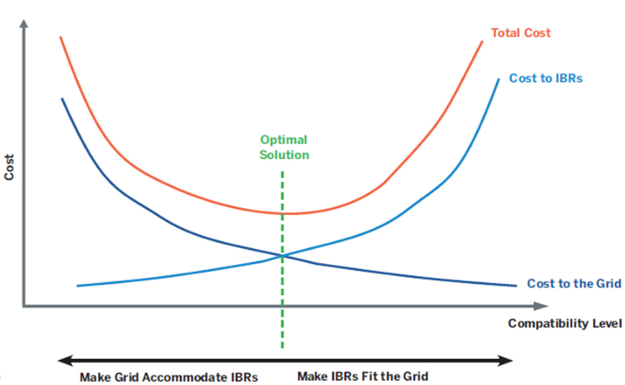
\includegraphics[width=0.85\textwidth]{figuras/coste_optimo_ers.png}
    \vspace{0.2cm}
    \caption[Optimización tecno-económica de la resiliencia en sistemas
    dominados por IBR.]{%
    Representación conceptual del coste total del sistema en función
    del nivel de penetración de IBR. El mínimo de coste total se
    alcanza con un mix que remunera los ERS, no con la simple
    maximización de la penetración renovable. Fuente: Adaptado de Julia
    Matevosyan (ESIG) / Plataforma FUTURED \cite{futured2024}}
    \label{fig:futured_coste_optimo}
\end{figure}

% =====================================================================
\section{La respuesta normativa: del P.O.~7.4 obsoleto al
\textit{grid-forming} obligatorio}
\label{sec:evolucion_normativa}
% =====================================================================

\subsection{Las deficiencias del marco preexistente}
\label{subsec:po74_previo}

El Procedimiento de Operación 7.4 vigente en el momento del apagón no
había sido revisado sustancialmente en aproximadamente veinticinco años
\cite{boe2025}. Concebido para un parque de generación de base síncrona,
presentaba dos deficiencias críticas ante la realidad del 28A. La primera
era la asimetría de participación: el grueso del parque renovable
---que cubría el 82~\% de la generación en el momento del colapso---
operaba con factor de potencia fijo, inhabilitado para inyectar o absorber
reactiva de forma dinámica. La segunda era la banda muerta: los
generadores síncronos convencionales estaban eximidos de actuar si la
tensión en la red de 400~kV se mantenía entre 405~kV y 410~kV,
configurando una respuesta por escalones que resultó estructuralmente
incompatible con la velocidad del transitorio capacitivo documentado
\cite{ree2025,icai2025}.

La respuesta regulatoria se articuló en tres capas sucesivas: la revisión
urgente del P.O.~7.4, las medidas de urgencia del Real Decreto 997/2025,
y la adaptación al nuevo código de red europeo NC~RfG~2.0.

\begin{figure}[H]
    \centering
    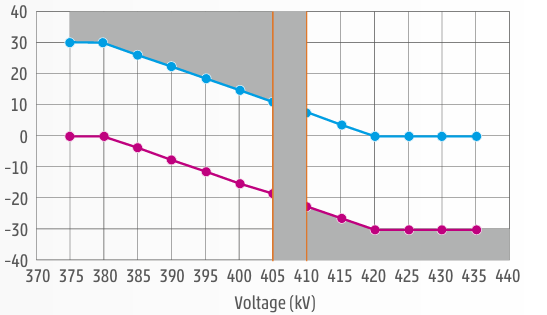
\includegraphics[width=0.85\textwidth]{figuras/po74_banda_muerta.png}
    \vspace{0.2cm}
    \caption[Limitaciones del control de tensión en el P.O.~7.4 original
    (banda muerta).]{%
    Curva característica de inyección/absorción de reactiva del antiguo
    P.O.~7.4. La zona sombreada ilustra la ``banda muerta'' entre 405~kV
    y 410~kV, rango en el cual el parque generador no estaba obligado a
    proveer respuesta dinámica, inhabilitando la defensa del sistema
    frente a transitorios capacitivos rápidos. Fuente: REE.}
    \label{fig:po74_bandamuerta}
\end{figure}

\subsection{La revisión del P.O.~7.4, el sistema VOLTAIRE y el nuevo
esquema retributivo}
\label{subsec:po74_voltaire}

La Resolución de la CNMC de 12 de junio de 2025 (BOE-A-2025-13076)
reformuló el P.O.~7.4 bajo el nuevo marco de servicios de no frecuencia
derivado del Reglamento (UE) de Balance Eléctrico. La innovación
fundamental del texto revisado es la sustitución del modelo de consignas
estáticas por una prestación dinámica retribuida: el seguimiento preciso
de \textit{setpoints} en tiempo real, enviados telemáticamente por el
Centro de Control Eléctrico (CECOEL) a través del Centro de Control de
Energías Renovables
(CECRE)\textsuperscript{\ref{anexo:cecre}} \cite{boe2025}.

El canal de comunicación entre CECOEL y el parque renovable se articula
a través del sistema VOLTAIRE\textsuperscript{\ref{anexo:voltaire}}: un
lazo de control proporcional-integral que opera en dos capas jerárquicas.
La Regulación Terciaria optimiza globalmente el perfil de tensiones a nivel
nacional mediante flujos de cargas óptimos reactivos. La Regulación
Secundaria envía consignas telemáticas en tiempo real con una resolución
de muestreo de 4~s, cerrando el bucle de control a escala de parque y
eliminando la dependencia de la respuesta manual del operador ante
transitorios de tensión de baja amplitud. Esta arquitectura transformó el
rol del parque renovable: de consumidor pasivo de la tensión de red a
actuador activo del sistema de regulación nacional \cite{boe2025}.

Para retribuir los costes de oportunidad de proveer reactiva y alinear
los incentivos económicos de los promotores, el marco actualizado
introduce las siguientes retribuciones: 2~\texteuro/MVArh para la
prestación en tiempo real durante horas con producción neta positiva; y
para horas con producción nula o negativa ---período nocturno en el que
el efecto Ferranti de las líneas descargadas genera sobretensiones
capacitivas--- una retribución indexada al Precio Medio Diario del
mercado mayorista mediante:

\begin{equation}
    r_Q = 0{,}05 \times 1{,}15 \times \mathrm{PMD} + 5
    \quad [\texteuro/\mathrm{MVArh}]
    \label{eq:retribucion_reactiva_nocturna}
\end{equation}

Los sistemas de almacenamiento BESS reciben adicionalmente un pago de
disponibilidad de 2{,}7~\texteuro/MW/día sobre la potencia instalada,
condicionado al mantenimiento de una tasa de cumplimiento de muestras
válidas superior al 90~\%.

\begin{table}[H]
    \centering
    \caption[Comparativa del servicio de control de tensión: P.O.~7.4
    original y marco actualizado (CNMC, 2025).]{%
    Comparativa técnica y regulatoria del servicio de control de
    tensión entre el P.O.~7.4 original y el marco actualizado tras
    el incidente. Fuente: Elaboración propia / \cite{boe2025}}
    \vspace{0.3cm}
    \begin{tabularx}{\textwidth}{@{} l >{\RaggedRight\arraybackslash}X
                                      >{\RaggedRight\arraybackslash}X @{}}
        \toprule
        \textbf{Atributo operativo}
            & \textbf{P.O.~7.4 original (pre-2025)}
            & \textbf{Marco actualizado (post-2025)} \\
        \midrule
        Naturaleza del control
            & Estática y asimétrica. Operación por escalones discretos.
            & Dinámica, continua y proporcional a la desviación. \\
        \addlinespace
        Participación IBR
            & \textit{Grid-following} pasivo con factor de potencia fijo.
              Sin respuesta dinámica.
            & \textit{Grid-forming} obligatorio. Participación activa en
              la consigna de tensión $V$. \\
        \addlinespace
        Banda muerta ($V$)
            & Rango de 405~kV a 410~kV sin respuesta obligatoria.
            & Eliminada o reducida a $\pm 0{,}5$~\% de $U_n$. \\
        \addlinespace
        Respuesta en reactiva
            & Escalones de consigna lenta tras petición del OS.
            & Respuesta automática en bucle cerrado (\textit{droop
              control}). \\
        \addlinespace
        Remuneración de $Q$
            & Basada en disponibilidad técnica declarada.
            & Retribuida mediante mercados zonales de servicios ERS. \\
        \addlinespace
        Observabilidad
            & Telemedidas SCADA de nudos de 400~kV, resolución de
              varios segundos.
            & Monitorización de alta resolución mediante PMU y
              telemedida de 4~s para IBR distribuidos. \\
        \addlinespace
        Régimen sancionador
            & Sin penalizaciones específicas por incumplimiento de
              consignas de reactiva.
            & Penalizaciones económicas por incumplimiento de la tasa
              de cumplimiento mínima del 90~\% de muestras válidas
              dentro de la ventana de evaluación mensual. \\
        \bottomrule
    \end{tabularx}
    \label{tab:comparativa_normativa_po74_v2}
\end{table}

El texto revisado del P.O.~7.4 endurece además las exigencias dinámicas
del control a nivel de planta: para variaciones de consigna con
diferencia de reactiva inferior a 50~MVAr, el tiempo de respuesta máximo
es de 2~min, el tiempo de establecimiento máximo de 5~min y el sobrepaso
máximo del 120~\% del salto solicitado. En la modalidad de seguimiento
de tensión (Modalidad~U), el proveedor debe escalar la inyección mediante
un limitador de rampa de 0{,}33~\% de $U_n$ por minuto \cite{boe2025}.

El Real Decreto 997/2025, de 5 de noviembre, complementó la reforma del
P.O.~7.4 con cuatro medidas de urgencia de rango reglamentario
\cite{rd997_2025}: la redefinición jurídica de los sistemas BESS como
activos de servicio de estabilidad sistémica, con acceso explícito a los
mercados de ERS; el saneamiento del registro de permisos de conexión
obsoletos, condición previa para la implantación de las subastas zonales
de capacidad de reactiva; la obligatoriedad de telemedida con resolución
inferior a 4~s para todo el parque IBR significativo, habilitando la
observabilidad necesaria para el control VOLTAIRE; y la obligatoriedad
del módulo de amortiguamiento de oscilaciones
(PSS/POD)\textsuperscript{\ref{anexo:pss_pod}} en todos los inversores
GFM de nueva instalación con potencia superior a 10~MW.

La tensión regulatoria generada por la evolución del P.O.~7.4 revela una
contradicción tecnológica que el propio proceso hizo visible: en octubre
de 2025, REE solicitó elevar la exigencia de cumplimiento del 75~\% al
90~\% del tiempo. La CNMC denegó la petición argumentando la
imposibilidad técnica de los grupos síncronos existentes para alcanzar
ese nivel de cumplimiento con las rampas de ajuste requeridas. El dato es
revelador en sentido inverso: los inversores GFM podrían cumplir sin
dificultad esa exigencia, mientras que las máquinas rotativas a las que
la norma originalmente iba destinada no pueden igualar la velocidad del
nuevo estándar. La adaptación del marco operativo a las capacidades de
los IBR-GFM avanza a mayor velocidad que la de los activos síncronos a
los que la norma sustituye como proveedores de servicios ancilares
\cite{boe2025}.

\subsection{El marco europeo: NC~RfG~2.0 y los Informes de Fase~I y
Fase~II de ENTSO-E}
\label{subsec:nc_rfg_20}

Mientras las medidas nacionales actuaban como respuestas operativas a
corto plazo, la respuesta sistémica orientada al futuro a escala
continental emana de la refundación del Código de Red de Requisitos para
Generadores (NC~RfG)\textsuperscript{\ref{anexo:nc_rfg}} por parte de
ENTSO-E.

El NC~RfG vigente en la última década fue diseñado bajo el paradigma GFL:
estandarizaba los perfiles de hueco y los umbrales de frecuencia, pero no
contemplaba la posibilidad de que no quedara ninguna máquina rotativa
pesada a la que seguir. Esta carencia conceptual quedó demostrada en los
8 segundos del colapso ibérico. El Grupo Técnico de ENTSO-E sobre
Capacidad de Formación de Red (TG~GFC) cristalizó su trabajo en dos
documentos de referencia:

\begin{itemize}
    \item \textbf{Informe de Fase~I (mayo de 2024):} Estableció la
    definición técnica fundamental del GFM requerida por el nuevo código:
    caracterización del comportamiento transitorio como ``fuente de
    tensión detrás de una reactancia efectiva constante'' durante los
    primeros milisegundos tras una perturbación. Este modelo fasorial
    proscribe de facto las dependencias directas de algoritmos PLL para
    el control primario de la corriente de falta.

    \item \textbf{Informe de Fase~II (noviembre de 2025):} Publicado bajo
    el peso de la evidencia del colapso ibérico, este documento obtuvo el
    aval transversal de los organismos industriales (CENELEC, WindEurope,
    SolarPower Europe, EASE). Establece de forma taxativa cómo las nuevas
    plantas de generación y los sistemas de almacenamiento basados en
    inversores deben estabilizar el sistema \cite{entsoe2025phase2}.
\end{itemize}

Las obligaciones GFM del NC~RfG~2.0, consolidadas en la
Recomendación~03-2023 de ACER y en el Informe de Fase~II, se aplican
con un enfoque tecnológicamente agnóstico: el código establece los
principios del servicio, delegando en cada TSO la especificación de los
parámetros operativos. La clasificación por tipos es la siguiente:

\begin{table}[H]
    \centering
    \caption[Clasificación de módulos según el NC~RfG~2.0 y requisito
    GFM asociado.]{%
    Tipos de módulos y requisitos de capacidad \textit{grid-forming}
    establecidos por el NC~RfG~2.0 y la Recomendación 03-2023 de ACER
    para el Área Síncrona de Europa Continental. Fuente: Elaboración
    propia / \cite{entsoe2025phase2} / \cite{acer2023}}
    \vspace{0.3cm}
    \small
    \begin{tabularx}{\textwidth}{>{\bfseries}p{1.8cm}
                                 >{\RaggedRight\arraybackslash}p{3.2cm}
                                 >{\RaggedRight\arraybackslash}X
                                 >{\centering\arraybackslash}p{2.5cm}}
    \toprule
    \textbf{Tipo} & \textbf{Potencia / Conexión}
                  & \textbf{Requisito GFM}
                  & \textbf{Cronograma} \\
    \midrule
    Tipo~A
        & $< 1$~MW
        & Voluntario. Sujeto al criterio del DSO.
        & N/A \\
    \addlinespace
    Tipo~B
        & 1--50~MW
        & Obligatorio. Inercia sintética y soporte dinámico básico de
          tensión.
        & Máx. 3 años tras publicación del IGD de ENTSO-E. \\
    \addlinespace
    Tipo~C
        & $> 50$~MW
        & Obligatorio y exhaustivo. Operación plena como fuente de
          tensión; perfiles de corriente de falta; funcionalidad POD.
        & 3 años tras adopción definitiva por la Comisión Europea. \\
    \addlinespace
    Tipo~D
        & $\geq 110$~kV o $> 75$~MW
        & Idéntico al Tipo~C más pruebas de certificación.
        & 3 años tras adopción definitiva por la Comisión Europea. \\
    \addlinespace
    ESM (BESS)
        & Según categoría
        & Ídem al módulo PPM equivalente. Los sistemas V2G con
          capacidad conjunta $> 1$~MW se clasifican como ESM Tipo~B.
        & Según categoría. \\
    \bottomrule
    \end{tabularx}
    \label{tab:nc_rfg_clasificacion}
\end{table}

Dado que ciertas arquitecturas de inversores GFM a gran escala se
encuentran en fase de maduración industrial, el NC~RfG~2.0 estipula un
período transitorio de un máximo de 3~años tras su entrada en vigor
durante el cual el requisito GFM actuará como no obligatorio. Las
Autoridades Nacionales de Regulación pueden acortar este período
atendiendo a las necesidades específicas de sus redes
\cite{acer2023,entsoe2025phase2}.

A la fecha de redacción del presente trabajo, la adopción formal del
NC~RfG~2.0 por la Comisión Europea se encuentra despriorizada y sin
calendario oficial, lo que genera una ventana de incertidumbre
regulatoria que los operadores nacionales están gestionando mediante
medidas preventivas al margen del código \cite{gobierno2025}.

% =====================================================================
\section{Mercados de Servicios Esenciales de Confiabilidad: la
traducción económica de la resiliencia}
\label{sec:mercados_ers}
% =====================================================================

\subsection{El problema del \textit{headroom}: por qué el mercado de
energía no remunera la estabilidad}
\label{subsec:headroom}

La transición hacia la filosofía GFM conlleva una fricción económica
estructural. Para que un inversor GFM pueda actuar como fuente de tensión
ante un RoCoF severo o una perturbación de tensión, debe mantener
obligatoriamente una reserva de su capacidad aparente ($S_{\max}$) no
utilizada en estado estacionario. Esta reserva ---denominada en la
literatura técnica \textit{headroom}\textsuperscript{\ref{anexo:headroom}}---
exige o bien limitar deliberadamente la potencia activa inyectada en el
mercado de energía diario, o bien sobredimensionar la etapa de potencia
de sus IGBT aumentando drásticamente el CAPEX. Sin compensación económica
directa, ninguna de estas opciones es viable comercialmente.

El fracaso estructural de la arquitectura regulatoria vigente hasta el
28A residía en su enfoque punitivo: penalizar las desviaciones técnicas
sin remunerar los atributos de firmeza. El nuevo corpus normativo
---P.O.~7.4 revisado y NC~RfG~2.0--- intenta corregir esta asimetría
mediante el diseño de mercados de ERS \cite{entsoe2025,gobierno2025}.

\subsection{Mecanismos de mercado: tres vectores de remuneración}
\label{subsec:ers_mecanismos}

Los informes post-28A y la literatura técnica establecen las directrices
para que los reguladores nacionales estructuren sistemas de remuneración
que eviten infraestructuras ociosas o desincentivos económicos. Las
propuestas se articulan en tres mecanismos complementarios
\cite{entsoe2025,gobierno2025}:

\vspace{0.3cm}
\noindent\textbf{1. Mercados regionales de inercia sintética y
contención rápida de frecuencia.}

El diseño ibérico y europeo avanzará hacia subastas donde se abone un
pago por capacidad o de disponibilidad a los activos capaces de proveer
soporte inercial en márgenes de tiempo inferiores a 5~milisegundos. La
lógica del mecanismo es la acumulación de fuentes de ingresos
(\textit{revenue stacking}): los sistemas BESS perciben ingresos
simultáneos de arbitraje de energía en el mercado diario, de las subastas
de regulación secundaria y terciaria de frecuencia, y de pagos por
capacidad de inercia sintética y por FFR. Esta multiplicidad de flujos
de ingresos compensa el elevado CAPEX del sobredimensionamiento de IGBT
y la pérdida de ingresos por el \textit{headroom} de reactiva.

\vspace{0.3cm}
\noindent\textbf{2. Señales geográficas de nivel de cortocircuito.}

A diferencia de la frecuencia ---una métrica global que se distribuye
instantáneamente por toda la zona síncrona continental---, el SCR y
las sobretensiones son fenómenos radicalmente locales y geográficamente
confinados. Los nudos vulnerables donde el colapso del SCR fue
documentado el 28A no coinciden con los nudos de mayor densidad de
potencia instalada. Por tanto, los mercados de ERS adoptarán señales de
precios espaciales granulares: tarifas de conexión descontadas o subastas
de capacidad de reactiva en los nudos perimetrales identificados
matemáticamente por los TSOs como enclaves con $\mathrm{SCR} < 2$.

Esta granularidad geográfica tiene una implicación práctica relevante
para la planificación: la ubicación de los BESS-GFM en los nudos correctos
pasa a ser determinante para la viabilidad económica del proyecto, ya que
los precios de los servicios ERS serán localmente más altos en las zonas
de mayor fragilidad sistémica.

\vspace{0.3cm}
\noindent\textbf{3. Remuneración ex-ante para inversiones puras de
estabilidad: compensadores síncronos.}

Para infraestructuras como los SynCons, que aportan inercia física pura
y corrientes de cortocircuito masivas pero no tienen capacidad de vender
energía en el mercado horario, la regulación contempla modelos de
retribución basados en el coste del servicio (\textit{Rate of Return
Regulation}), sin exposición al riesgo de precio de la energía, o
adjudicaciones a largo plazo que blindan la inversión de capital y
aseguran al Operador del Sistema una base rotatoria fiable con
independencia de la penetración instantánea de IBR-GFM
\cite{gobierno2025,entsoe2025}.

\begin{figure}[H]
    \centering
    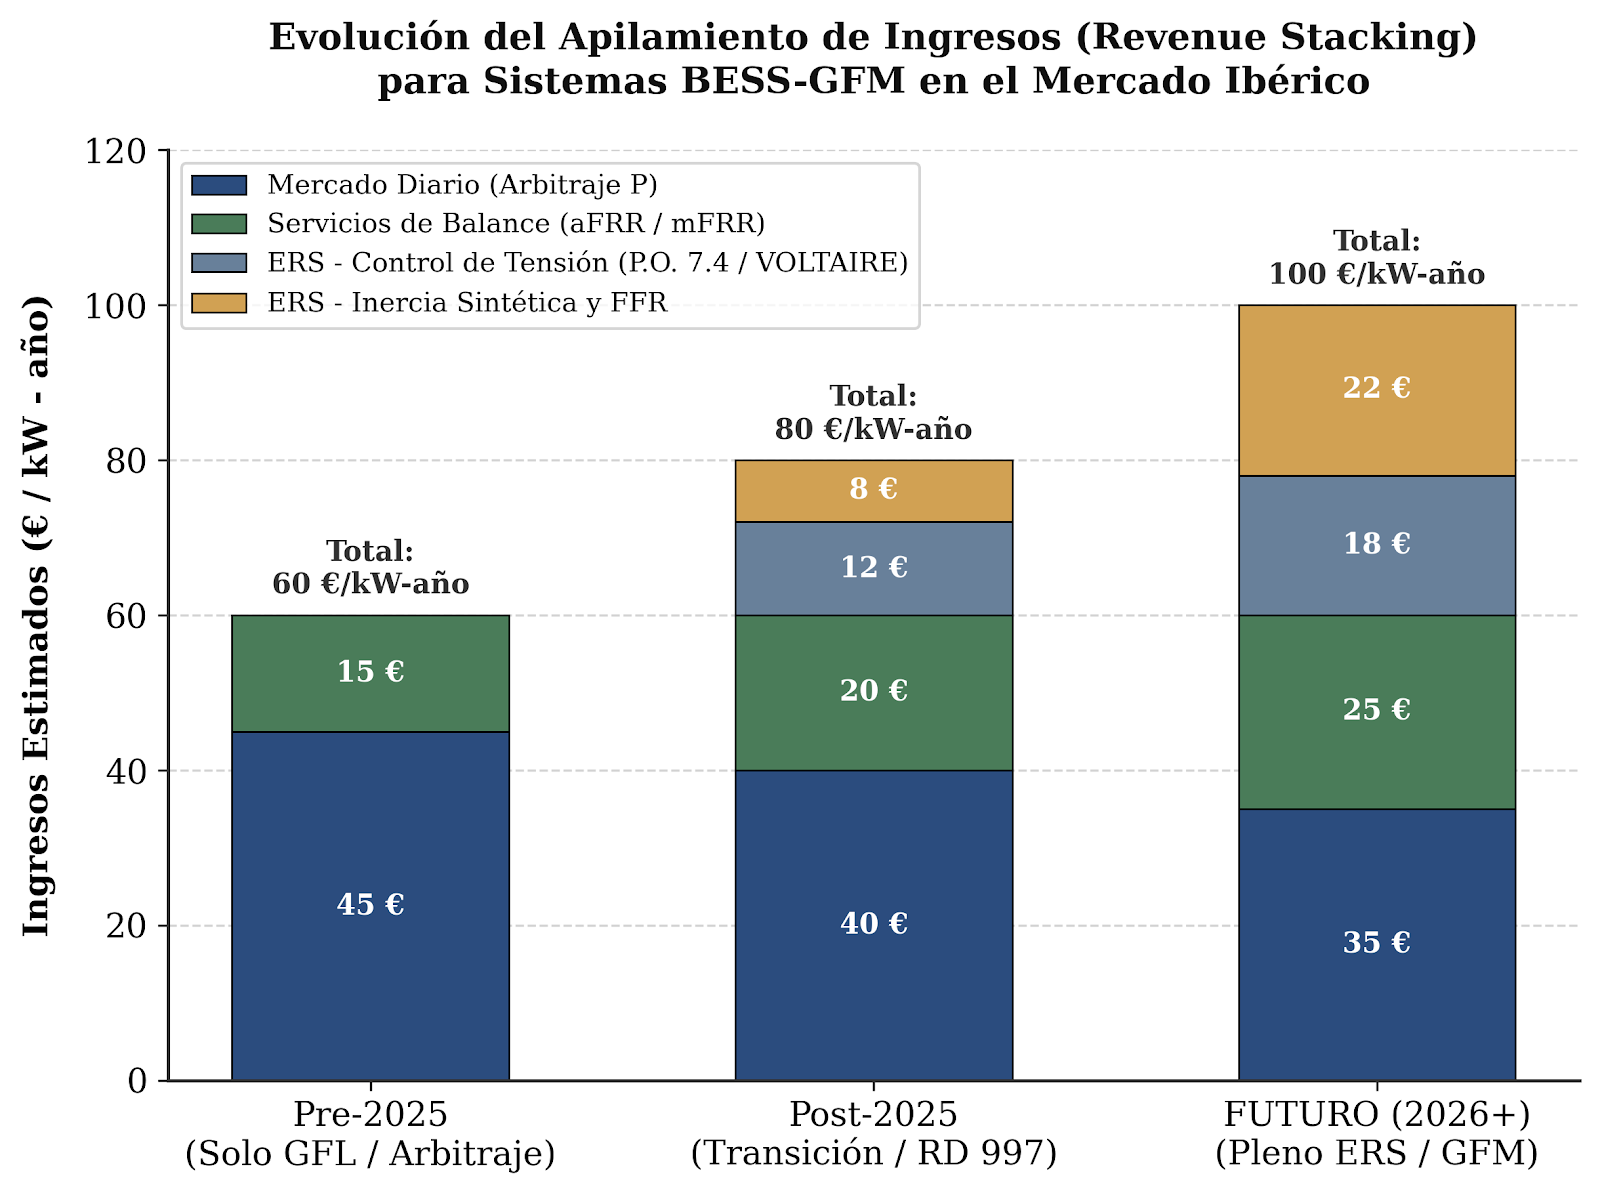
\includegraphics[width=0.85\textwidth]{figuras/ers_revenue_stacking.png}
    \vspace{0.2cm}
    \caption[\textit{Revenue stacking} en el nuevo marco de mercados ERS
    para sistemas BESS-GFM.]{%
    Diagrama de fuentes de ingresos apiladas para un sistema BESS-GFM
    bajo el marco regulatorio post-28A: mercado de energía diario,
    mercados de balance de frecuencia (aFRR/mFRR), subastas de inercia
    sintética y FFR, y pagos por disponibilidad de reactiva ERS.
    Fuente: Elaboración propia basada en la estructura de ENTSO-E
    \cite{entsoe2025_storage}.}
    \label{fig:revenue_stacking}
\end{figure}

\subsection{Los modelos de referencia: DS3 de EirGrid y RRS-FFR de ERCOT}
\label{subsec:ds3_ercot}

Los sistemas de EirGrid (Irlanda) y ERCOT (Texas) constituyen las
referencias operativas contrastadas hacia las que converge el diseño
europeo de los mercados ERS: ambos operadores han enfrentado con
antelación los desafíos de penetraciones de generación no síncrona
superiores al 75~\%.

El programa \textit{Delivering a Secure, Sustainable Electricity System}
(DS3)\textsuperscript{\ref{anexo:ds3}} de EirGrid fragmentó la provisión
de estabilidad en 14~productos altamente especializados. La
Tabla~\ref{tab:eirgrid_ds3} recoge los tres más relevantes para el
contexto del 28A.

\begin{table}[H]
\centering
\caption[Definiciones técnicas del programa DS3 de EirGrid.]{%
Definiciones técnicas y métricas de evaluación de los tres servicios
principales del programa DS3 de EirGrid relevantes para el contexto del
28A. Fuente: EirGrid / Elaboración propia}
\label{tab:eirgrid_ds3}
\vspace{0.3cm}
\small
\begin{tabularx}{\textwidth}{>{\bfseries}p{3.2cm} X
                             >{\centering\arraybackslash}p{4.5cm}}
\toprule
\textbf{Servicio} & \textbf{Definición técnica}
                  & \textbf{Umbral / Ventana} \\
\midrule
Synchronous Inertial Response (SIR)
    & Provisión casi instantánea de potencia activa y par sincronizante
      ante caídas de frecuencia. Se remunera mediante el índice
      $\mathrm{SIRF} = E_k / P_\mathrm{min}$, que penaliza el despacho
      de plantas ineficientes que inyectan potencia activa no deseada
      solo para aportar inercia marginal.
    & $\mathrm{SIRF} \geq 15$~s \\
\addlinespace
Fast Frequency Response (FFR)
    & Inyección rápida de potencia activa tras un evento de caída
      abrupta de frecuencia. La energía validable se calcula como la
      integral de la potencia adicional inyectada en los primeros 10~s
      ($T_0 \to T{+}10\,\mathrm{s}$). Se exige que la energía provista
      sea estrictamente mayor que la pérdida de energía incurrida en la
      recuperación ($T{+}10\,\mathrm{s} \to T{+}20\,\mathrm{s}$).
    & Respuesta entre 0{,}15~s y 2~s;
      $E_{\mathrm{prov}} > E_{\mathrm{loss}}$ \\
\addlinespace
Steady-State Reactive Power (SSRP)
    & Rango total de potencia reactiva despachable ($Q_{\mathrm{range}}$,
      en MVAr) que el inversor puede inyectar o absorber en operación
      continua a lo largo de su rango completo de potencia activa
      ($P_{\mathrm{range}}$). Incluye un escalar retributivo favorable
      para IBR capaces de proveer reactiva en vacío
      (\textit{watt-less VARs}).
    & Estado estacionario; valoración anual mediante modelos PLEXOS \\
\bottomrule
\end{tabularx}
\end{table}

El mercado RRS-FFR de ERCOT, descrito en la
sección~\ref{sec:tecnologias_habilitadoras}, complementa el modelo DS3
desde una perspectiva centrada en la respuesta de frecuencia subcíclica.
La comparación entre ambos sistemas sugiere una arquitectura de mercados
ERS de doble capa para el contexto europeo: una capa de señales
geográficas de cortocircuito ---análoga al SSRP de EirGrid--- y una capa
de respuesta de frecuencia subcíclica ---análoga al RRS-FFR de ERCOT.

\subsection{La evolución del marco español en 2026: P.O.~7.4 y P.O.~14.4}
\label{subsec:cnmc_2026}

La evolución regulatoria ha continuado en 2026. El 8 de mayo de 2026,
la CNMC abrió un trámite de audiencia pública para la modificación de los
Procedimientos de Operación P.O.~7.4 y P.O.~14.4 (Expediente
DCOOR/DE/006/26), orientado a la creación de mercados zonales de
servicios de no frecuencia con participación activa de IBR y BESS.

La lección estructural que el 28 de abril de 2025 inscribe en el diseño
regulatorio europeo es de alcance mayor que el de cualquier ajuste
incremental a los procedimientos de operación: los atributos físicos que
los sistemas síncronos aportaban de forma inherente ---inercia, potencia
de cortocircuito, control autónomo de tensión--- han dejado de ser
externalidades gratuitas para convertirse en servicios cuya provisión
debe ser definida, verificada y remunerada explícitamente. Como señalan
tanto el Comité de Análisis del Consejo de Seguridad Nacional como
ENTSO-E, el modelo marginalista puro de energía es estructuralmente
incapaz de remunerar esos atributos \cite{gobierno2025,entsoe2025}. Sin
esa traducción económica de la resiliencia, ninguna exigencia técnica
del NC~RfG~2.0 resultará sostenible en el medio plazo.